\documentclass[12pt]{article}
\usepackage[top=1in, bottom=1in, left=1in, right=1in]{geometry}

\usepackage{setspace}
\onehalfspacing

\usepackage{amssymb}
%% The amsthm package provides extended theorem environments
\usepackage{amsthm}
\usepackage{epsfig}
\usepackage{times}
\renewcommand{\ttdefault}{cmtt}
\usepackage{amsmath}
\usepackage{graphicx} % for graphics files

% Draw figures yourself
\usepackage{tikz} 

% writing elements
\usepackage{mhchem}

% The float package HAS to load before hyperref
\usepackage{float} % for psuedocode formatting
\usepackage{xspace}

% from Denovo Methods Manual
\usepackage{mathrsfs}
\usepackage[mathcal]{euscript}
\usepackage{color}
\usepackage{array}

\usepackage[pdftex]{hyperref}
\usepackage[parfill]{parskip}

% math syntax
\newcommand{\nth}{n\ensuremath{^{\text{th}}} }
\newcommand{\ve}[1]{\ensuremath{\mathbf{#1}}}
\newcommand{\Macro}{\ensuremath{\Sigma}}
\newcommand{\rvec}{\ensuremath{\vec{r}}}
\newcommand{\omvec}{\ensuremath{\hat{\Omega}}}
\newcommand{\vOmega}{\ensuremath{\hat{\Omega}}}
%---------------------------------------------------------------------------
%---------------------------------------------------------------------------
\begin{document}
\begin{center}
{\bf NE 155/255, Fall 2019 \\
Nuclear Physics Terms, continued\\
September 11, 2019}
\end{center}

\setlength{\unitlength}{1in}
\begin{picture}(6,.1) 
\put(0,0) {\line(1,0){6.25}}         
\end{picture}

\begin{enumerate}
\setcounter{enumi}{2}

\item \textbf{double-differential scattering x-sec}
      ($\sigma_s(E, \vOmega \rightarrow E', \vOmega')dE' d\vOmega'$): measure 
      of the probability that a neutron of energy $E$ and moving in direction
      $\vOmega$ scatters off of a specific nucleus into energy range
      $[E', E' + dE']$ and direction range $[\vOmega', \vOmega' + d\vOmega']$.

We can think of this as the fractional probability multiplied by the total 
scattering cross section

\begin{align*}
\sigma_s(E, \vOmega \rightarrow E', \vOmega') &=
\sigma_s(E) f_s(E, \vOmega \rightarrow E', \vOmega')\\
\text{where } &\int_0^{E_0} dE' \int_{4 \pi} d\vOmega' \:
f_s(E, \vOmega \rightarrow E', \vOmega') = 1 \\
\sigma_s(E) &= \int_0^{E_0} dE' \int_{4 \pi} d\vOmega' \:
\sigma_s(E, \vOmega \rightarrow E', \vOmega')
\end{align*}

\item \textbf{fission yield} ($\nu(E)$): average \# of neutrons released by a 
      fission induced by a neutron of energy E.

\item \textbf{fission spectrum} ($\chi(E)dE$): average \# of neutrons produced 
      from fission that are born with energy in $[E, E + dE]$. This is 
      normalized such that \[\int_0^{\infty} \chi(E)dE =1\:.\]

\begin{itemize}
\item U-235: $\chi(E) = 0.453 e^{-1.036E} \sinh(\sqrt{2.29E})$
\item Pu-239: $\chi(E) = 0.6739 \sqrt{E} e^{-E / 1.41}$
\end{itemize}

\item \textbf{particle angular density}
      ($n(\vec{r}, E, \vOmega, t)d\vec{r} d\vOmega dE$): expected number of 
      particles in volume element $d^3r$ at $\vec{r}$ whose energies are in
      $[E, E + dE]$ and direction of motion is in
      $[\vOmega, \vOmega + d\vOmega]$ at time $t$.

Note:

\begin{align*}
n(\vec{r}, E, \vOmega, t) &= \frac{1}{mv}n(\vec{r}, v, \vOmega, t) \\
n(\vec{r}, v, \vOmega, t) &= v^2 n(\vec{r}, \vec{v}, t) \\
n(\vec{r}, \vec{v}, t) &= \frac{m}{v}n(\vec{r}, E, \vOmega, t)
\end{align*}
\begin{figure}[h!]
    \begin{center}
    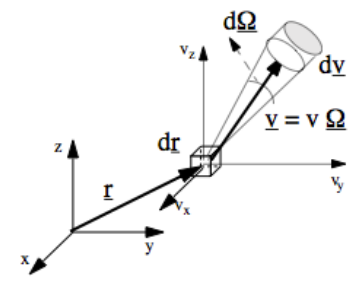
\includegraphics[keepaspectratio, width = 2.5 in]{differential-element}
    \end{center}
    \caption{Differential volume, velocity (energy), and angle}
    \label{fig:differential}
\end{figure}

\item \textbf{particle density}: ($N(\vec{r},E,t)d^3r dE$): expected number of 
      particles in $d^3r$ at $\vec{r}$ whose energies are in $[E, E + dE]$ at 
      time $t$.

\[N(\vec{r},E,t)d^3r dE =
\int_{4\pi} d\vOmega\: n(\vec{r}, E, \vOmega, t)d^3r dE \]

\item \textbf{angular flux}:
      $\psi(\vec{r}, E, \vOmega, t) \equiv v n(\vec{r}, E, \vOmega, t)$
      [neutrons / (cm$^2$ s MeV steradian)] can be thought of as path length 
      per unit volume about $\vec{r}$ passed by neutrons with energies...

\item \textbf{scalar flux}: $\phi(\vec{r},E,t) \equiv v N(\vec{r},E,t)$ 
      [neutrons / (cm$^2$ s MeV)] can be thought of as the number of neutrons 
      that penetrate a sphere of 1 cm$^2$ cross sectional area at $\vec{r}$ 
      with energies in $dE$ about $E$ at time $t$.

\[= \int_{4\pi} d\vOmega\: \psi(\vec{r}, E, \vOmega, t) \]

\item \textbf{interaction rate density}: expected number of $j$ reactions per 
volume per energy at time $t$.

\[\int_{4\pi} d\vOmega \:\Sigma_j v n(\vec{r}, E, \vOmega, t) =
\Sigma_j \phi(\vec{r},E,t)\]

\item \textbf{angular current density} or partial current:
      $\vec{j}(\vec{r}, E, \vOmega, t) = \vec{v} n(\vec{r}, E, \vOmega, t)$; 

$\vec{j}(\vec{r}, E, \vOmega, t) \cdot \hat{e}\: dA\: dE\: d\vOmega$ is the 
expected number of particles crossing $dA$ per second along unit direction
$\hat{e}$ with energy in $[E, E + dE]$ and direction in
$[\vOmega, \vOmega + d\vOmega]$ at time $t$.

\item \textbf{net current}: $\vec{J}(\vec{r}, E, t) $ is the net \# of 
      particles crossing a unit area per second along a direction normal to 
      that area with energies in $[E, E + dE]$ at time $t$.

\[\vec{J}(\vec{r}, E, t) = \int_{4\pi} d\vOmega\:
\vOmega \psi(\vec{r}, E, \vOmega, t)\]

\end{enumerate}

\end{document}
